% Dette afsnit skal handle om oversvømmelsers konsekvenser og progonoser. Ikke om nogen specifik type af oversvømmelse endnu.

\section{Oversvømmelser nu og i fremtiden}\label{sc:oversvoemmelser}
I dette afsnit bliver der fundet frem til projektets fokuspunkt. Dette fokuspunkt analyseres ved hjælp af et problemtræ \cite{3}. Ud fra problemtræet vil der blive vurderet, hvilke områder projektet vil have fokus på i forhold til en mulig løsning.

\subsection{Stormfloder i Danmark}
En naturkatastrofe er en katastrofe som sker naturligt og derfor ikke er forårsaget af mennesker. Dette kunne eksempelvis være tornadoer, jordskælv, vulkanudbrud eller oversvømmelser. Skader forårsaget af naturkatastrofer kan koste penge og menneskeliv \cite{3a}.
%https://www.basicplanet.com/natural-disasters/
Projektets fokus rettes mod det centrale problem som lyder \textit{“Stormfloder i Danmark”}, da stormfloder forekommer i Danmark. Dette er et problem, fordi stormfloder leder til skader. Dette ses eksempelvis på den stormflod, som i november 2016 ramte Danmark og resulterede i 3.941 anmeldte skader\cite{3b}.
\par
Dette centrale problem er analyseret ved hjælp af førnævnte problemtræ. Hertil er der udvalgt emner, som bliver analyseret og dokumenteret på baggrund af relevans og danner følgende træ i figur \ref{Problemtrae}.
%%%%
\begin{figure}[H]
    \centering
    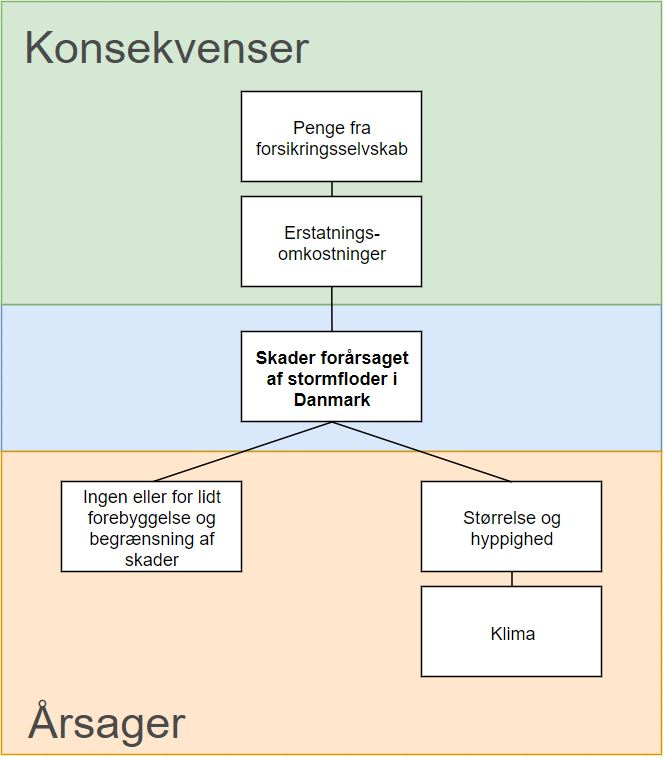
\includegraphics[width=0.7\textwidth]{figures/problemTrae.JPG}
    \caption{Problemtræsdiagram af projektets udvalgte emner, som bliver dokumenteret. Problemtræet givet et visuelt billede af årsager og konsekvenser omkring det centrale problem}
    \label{Problemtrae}
\end{figure}
%%%%

\subsubsection{Konsekvenser}
Statistik fra Stormrådet oplyser tal på de skader og omkostninger, som stormfloder har forvoldt i årene 1991 til 2008. Ifølge statistikken er der igennem de nævnte år udbetalt over 550 mio. kr. i stormflodsskader, altså ca. 32,3 mio. kr. om året \cite{3b}.
%https://www.stormraadet.dk/media/19385/stormflod-skadesstatistik-1991-2008.pdf
Selve behandlingen af en skade sker gennem forsikringsselskabet, hvor den skadelidte har sin brandforsikring. Forsikringsselskabet har her ansvar for kommunikation, taksering og afgørelse om skaden skal dækkes \cite{3c}.
%https://www.stormraadet.dk/media/54282/stormraadetsaarsberetning2018.pdf

\subsubsection{Årsager}
Stormfloder opstår på grund af en for høj vandstand. Dette kan skyldes tidevand, lufttryk eller vindafstivning, hvor Kystdirektoratet har målt effekten af disse i Thorsminde. Tidevand er et resultat af tiltrækningskraften mellem Jorden og Månen og vil i springtid og niptid forhøje vandstanden. Springtid sker når sol og måne står på linje og eksempelvis giver fuldmåne eller nymåne. Det giver en højere vandstand på omkring 0,3 meter. Niptid er derimod når solen og månen står vinkelret på hinanden og giver halvmåne, som resulterer i en forhøjelse på omkring 0,2 meter. 
\par 
Et fald i lufttrykket vil som sagt også resultere i en forhøjet vandstand. Lufttrykket ligger i gennemsnit på 1013 hPa (hektopascal). I stormvejr kan trykket falde til 970 hPa, hvilket vil forøge vandestanden med omkring 0,3 meter. 
\par 
Endeligt vil vindstuvning også påvirke vandstanden. Dette skyldes vindens pres på vandoverfladen, og har størst effekt på lave vanddybder. Vandstanden i Thorsminde kan eksempelvis komme op på en forhøjelse på 3 meter \cite{3d}.
%http://kysterne.kyst.dk/hvad-er-en-stormflod.html
\par
Der er også tale om at vandstanden stiger på grund af klimaforandring. En relevant interessent inden for området er “The Intergovernmental Panel on Climate Change” (IPCC) som er Forenede Nationers (FN) klimapanel. Her argumenterer IPCC for at vandstanden bliver højere, grundet smeltning af gletsjere \cite{3e}.
% https://www.ipcc.ch/site/assets/uploads/2018/02/WG1AR5_Chapter13_FINAL.pdf
Videnskab.dk har formidlet IPCC prognoser for vandstanden i fremtiden ved følgende tabel:
%%%%
\begin{figure}[H]
    \centering
    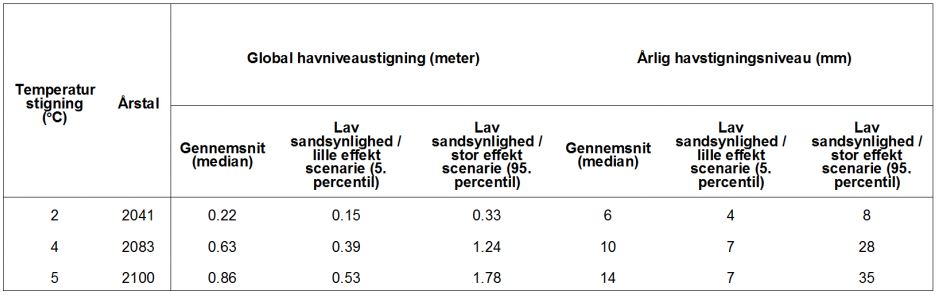
\includegraphics[width=0.7\textwidth]{figures/IPCC.JPG}
    \caption{Forventet havstigning og hastighed af havstigningen hvis de globale temperaturer stiger med 2, 4 og 5 grader, når vi når frem til henholdsvis år 2041, 2083 og 2100 . (Data: Jevrejeva et a. 2016) \cite{}}
    \label{Havstigning}
\end{figure}
%%%%
Her forudser IPCC at den globale vandstand kan være forøget med 0,22 meter i 2041 \cite{3f}. % https://videnskab.dk/naturvidenskab/spaadom-forvaerret-saa-meget-stiger-havet
Dette kan resultere i, at det er nemmere at få stormfloder i Danmark som derfor også kan ske hyppigere og have større effekt.
\par
Skader forårsaget af stormfloder kan også forebygges eller begrænses. En anbefaling fra Kystdirektoratet fortæller, at den skadelidte bør gøre dette med mål om, at forhindre vand at komme ind \cite{3g}. Dette betyder at den skadelidte begrænser mængden af skader.
%http://kysterne.kyst.dk/stormraadet.html

\subssection{Delkonklussion}
Projektets fokus afgrænses til forebyggelse og begrænsning af skader forårsaget af stormfloder i Danmark. Denne afgrænsning sker på baggrund af, at der er potentiale for metoder, som bedre kan forebygge og begrænse skader. Dette er også et relevant område, da den globale havoverflade stiger i takt med at gletsjere smelter. Det resulterer i, at stormfloder kan forekomme hyppigere og med større effekt. En løsning som formindsker skader, vil også formindske forsikringsselskabernes omkostninger, som bruges på at dække stormflodskader. I næste kapitel bliver det undersøgt, hvilke muligheder der er for at formindske mængden af skader, som stormfloder forårsager. Derefter bliver der fundet frem til, hvordan en løsning kommer til at fungere, samt hvordan løsningen skal formindske disse skader.